
% Default to the notebook output style

    


% Inherit from the specified cell style.




    
\documentclass[11pt]{article}

    
    
    \usepackage[T1]{fontenc}
    % Nicer default font (+ math font) than Computer Modern for most use cases
    \usepackage{mathpazo}

    % Basic figure setup, for now with no caption control since it's done
    % automatically by Pandoc (which extracts ![](path) syntax from Markdown).
    \usepackage{graphicx}
    % We will generate all images so they have a width \maxwidth. This means
    % that they will get their normal width if they fit onto the page, but
    % are scaled down if they would overflow the margins.
    \makeatletter
    \def\maxwidth{\ifdim\Gin@nat@width>\linewidth\linewidth
    \else\Gin@nat@width\fi}
    \makeatother
    \let\Oldincludegraphics\includegraphics
    % Set max figure width to be 80% of text width, for now hardcoded.
    \renewcommand{\includegraphics}[1]{\Oldincludegraphics[width=.8\maxwidth]{#1}}
    % Ensure that by default, figures have no caption (until we provide a
    % proper Figure object with a Caption API and a way to capture that
    % in the conversion process - todo).
    \usepackage{caption}
    \DeclareCaptionLabelFormat{nolabel}{}
    \captionsetup{labelformat=nolabel}

    \usepackage{adjustbox} % Used to constrain images to a maximum size 
    \usepackage{xcolor} % Allow colors to be defined
    \usepackage{enumerate} % Needed for markdown enumerations to work
    \usepackage{geometry} % Used to adjust the document margins
    \usepackage{amsmath} % Equations
    \usepackage{amssymb} % Equations
    \usepackage{textcomp} % defines textquotesingle
    % Hack from http://tex.stackexchange.com/a/47451/13684:
    \AtBeginDocument{%
        \def\PYZsq{\textquotesingle}% Upright quotes in Pygmentized code
    }
    \usepackage{upquote} % Upright quotes for verbatim code
    \usepackage{eurosym} % defines \euro
    \usepackage[mathletters]{ucs} % Extended unicode (utf-8) support
    \usepackage[utf8x]{inputenc} % Allow utf-8 characters in the tex document
    \usepackage{fancyvrb} % verbatim replacement that allows latex
    \usepackage{grffile} % extends the file name processing of package graphics 
                         % to support a larger range 
    % The hyperref package gives us a pdf with properly built
    % internal navigation ('pdf bookmarks' for the table of contents,
    % internal cross-reference links, web links for URLs, etc.)
    \usepackage{hyperref}
    \usepackage{longtable} % longtable support required by pandoc >1.10
    \usepackage{booktabs}  % table support for pandoc > 1.12.2
    \usepackage[inline]{enumitem} % IRkernel/repr support (it uses the enumerate* environment)
    \usepackage[normalem]{ulem} % ulem is needed to support strikethroughs (\sout)
                                % normalem makes italics be italics, not underlines
    

    
    
    % Colors for the hyperref package
    \definecolor{urlcolor}{rgb}{0,.145,.698}
    \definecolor{linkcolor}{rgb}{.71,0.21,0.01}
    \definecolor{citecolor}{rgb}{.12,.54,.11}

    % ANSI colors
    \definecolor{ansi-black}{HTML}{3E424D}
    \definecolor{ansi-black-intense}{HTML}{282C36}
    \definecolor{ansi-red}{HTML}{E75C58}
    \definecolor{ansi-red-intense}{HTML}{B22B31}
    \definecolor{ansi-green}{HTML}{00A250}
    \definecolor{ansi-green-intense}{HTML}{007427}
    \definecolor{ansi-yellow}{HTML}{DDB62B}
    \definecolor{ansi-yellow-intense}{HTML}{B27D12}
    \definecolor{ansi-blue}{HTML}{208FFB}
    \definecolor{ansi-blue-intense}{HTML}{0065CA}
    \definecolor{ansi-magenta}{HTML}{D160C4}
    \definecolor{ansi-magenta-intense}{HTML}{A03196}
    \definecolor{ansi-cyan}{HTML}{60C6C8}
    \definecolor{ansi-cyan-intense}{HTML}{258F8F}
    \definecolor{ansi-white}{HTML}{C5C1B4}
    \definecolor{ansi-white-intense}{HTML}{A1A6B2}

    % commands and environments needed by pandoc snippets
    % extracted from the output of `pandoc -s`
    \providecommand{\tightlist}{%
      \setlength{\itemsep}{0pt}\setlength{\parskip}{0pt}}
    \DefineVerbatimEnvironment{Highlighting}{Verbatim}{commandchars=\\\{\}}
    % Add ',fontsize=\small' for more characters per line
    \newenvironment{Shaded}{}{}
    \newcommand{\KeywordTok}[1]{\textcolor[rgb]{0.00,0.44,0.13}{\textbf{{#1}}}}
    \newcommand{\DataTypeTok}[1]{\textcolor[rgb]{0.56,0.13,0.00}{{#1}}}
    \newcommand{\DecValTok}[1]{\textcolor[rgb]{0.25,0.63,0.44}{{#1}}}
    \newcommand{\BaseNTok}[1]{\textcolor[rgb]{0.25,0.63,0.44}{{#1}}}
    \newcommand{\FloatTok}[1]{\textcolor[rgb]{0.25,0.63,0.44}{{#1}}}
    \newcommand{\CharTok}[1]{\textcolor[rgb]{0.25,0.44,0.63}{{#1}}}
    \newcommand{\StringTok}[1]{\textcolor[rgb]{0.25,0.44,0.63}{{#1}}}
    \newcommand{\CommentTok}[1]{\textcolor[rgb]{0.38,0.63,0.69}{\textit{{#1}}}}
    \newcommand{\OtherTok}[1]{\textcolor[rgb]{0.00,0.44,0.13}{{#1}}}
    \newcommand{\AlertTok}[1]{\textcolor[rgb]{1.00,0.00,0.00}{\textbf{{#1}}}}
    \newcommand{\FunctionTok}[1]{\textcolor[rgb]{0.02,0.16,0.49}{{#1}}}
    \newcommand{\RegionMarkerTok}[1]{{#1}}
    \newcommand{\ErrorTok}[1]{\textcolor[rgb]{1.00,0.00,0.00}{\textbf{{#1}}}}
    \newcommand{\NormalTok}[1]{{#1}}
    
    % Additional commands for more recent versions of Pandoc
    \newcommand{\ConstantTok}[1]{\textcolor[rgb]{0.53,0.00,0.00}{{#1}}}
    \newcommand{\SpecialCharTok}[1]{\textcolor[rgb]{0.25,0.44,0.63}{{#1}}}
    \newcommand{\VerbatimStringTok}[1]{\textcolor[rgb]{0.25,0.44,0.63}{{#1}}}
    \newcommand{\SpecialStringTok}[1]{\textcolor[rgb]{0.73,0.40,0.53}{{#1}}}
    \newcommand{\ImportTok}[1]{{#1}}
    \newcommand{\DocumentationTok}[1]{\textcolor[rgb]{0.73,0.13,0.13}{\textit{{#1}}}}
    \newcommand{\AnnotationTok}[1]{\textcolor[rgb]{0.38,0.63,0.69}{\textbf{\textit{{#1}}}}}
    \newcommand{\CommentVarTok}[1]{\textcolor[rgb]{0.38,0.63,0.69}{\textbf{\textit{{#1}}}}}
    \newcommand{\VariableTok}[1]{\textcolor[rgb]{0.10,0.09,0.49}{{#1}}}
    \newcommand{\ControlFlowTok}[1]{\textcolor[rgb]{0.00,0.44,0.13}{\textbf{{#1}}}}
    \newcommand{\OperatorTok}[1]{\textcolor[rgb]{0.40,0.40,0.40}{{#1}}}
    \newcommand{\BuiltInTok}[1]{{#1}}
    \newcommand{\ExtensionTok}[1]{{#1}}
    \newcommand{\PreprocessorTok}[1]{\textcolor[rgb]{0.74,0.48,0.00}{{#1}}}
    \newcommand{\AttributeTok}[1]{\textcolor[rgb]{0.49,0.56,0.16}{{#1}}}
    \newcommand{\InformationTok}[1]{\textcolor[rgb]{0.38,0.63,0.69}{\textbf{\textit{{#1}}}}}
    \newcommand{\WarningTok}[1]{\textcolor[rgb]{0.38,0.63,0.69}{\textbf{\textit{{#1}}}}}
    
    
    % Define a nice break command that doesn't care if a line doesn't already
    % exist.
    \def\br{\hspace*{\fill} \\* }
    % Math Jax compatability definitions
    \def\gt{>}
    \def\lt{<}
    % Document parameters
    \title{01\_Intro\_to\_Jupyter}
    
    
    

    % Pygments definitions
    
\makeatletter
\def\PY@reset{\let\PY@it=\relax \let\PY@bf=\relax%
    \let\PY@ul=\relax \let\PY@tc=\relax%
    \let\PY@bc=\relax \let\PY@ff=\relax}
\def\PY@tok#1{\csname PY@tok@#1\endcsname}
\def\PY@toks#1+{\ifx\relax#1\empty\else%
    \PY@tok{#1}\expandafter\PY@toks\fi}
\def\PY@do#1{\PY@bc{\PY@tc{\PY@ul{%
    \PY@it{\PY@bf{\PY@ff{#1}}}}}}}
\def\PY#1#2{\PY@reset\PY@toks#1+\relax+\PY@do{#2}}

\expandafter\def\csname PY@tok@w\endcsname{\def\PY@tc##1{\textcolor[rgb]{0.73,0.73,0.73}{##1}}}
\expandafter\def\csname PY@tok@c\endcsname{\let\PY@it=\textit\def\PY@tc##1{\textcolor[rgb]{0.25,0.50,0.50}{##1}}}
\expandafter\def\csname PY@tok@cp\endcsname{\def\PY@tc##1{\textcolor[rgb]{0.74,0.48,0.00}{##1}}}
\expandafter\def\csname PY@tok@k\endcsname{\let\PY@bf=\textbf\def\PY@tc##1{\textcolor[rgb]{0.00,0.50,0.00}{##1}}}
\expandafter\def\csname PY@tok@kp\endcsname{\def\PY@tc##1{\textcolor[rgb]{0.00,0.50,0.00}{##1}}}
\expandafter\def\csname PY@tok@kt\endcsname{\def\PY@tc##1{\textcolor[rgb]{0.69,0.00,0.25}{##1}}}
\expandafter\def\csname PY@tok@o\endcsname{\def\PY@tc##1{\textcolor[rgb]{0.40,0.40,0.40}{##1}}}
\expandafter\def\csname PY@tok@ow\endcsname{\let\PY@bf=\textbf\def\PY@tc##1{\textcolor[rgb]{0.67,0.13,1.00}{##1}}}
\expandafter\def\csname PY@tok@nb\endcsname{\def\PY@tc##1{\textcolor[rgb]{0.00,0.50,0.00}{##1}}}
\expandafter\def\csname PY@tok@nf\endcsname{\def\PY@tc##1{\textcolor[rgb]{0.00,0.00,1.00}{##1}}}
\expandafter\def\csname PY@tok@nc\endcsname{\let\PY@bf=\textbf\def\PY@tc##1{\textcolor[rgb]{0.00,0.00,1.00}{##1}}}
\expandafter\def\csname PY@tok@nn\endcsname{\let\PY@bf=\textbf\def\PY@tc##1{\textcolor[rgb]{0.00,0.00,1.00}{##1}}}
\expandafter\def\csname PY@tok@ne\endcsname{\let\PY@bf=\textbf\def\PY@tc##1{\textcolor[rgb]{0.82,0.25,0.23}{##1}}}
\expandafter\def\csname PY@tok@nv\endcsname{\def\PY@tc##1{\textcolor[rgb]{0.10,0.09,0.49}{##1}}}
\expandafter\def\csname PY@tok@no\endcsname{\def\PY@tc##1{\textcolor[rgb]{0.53,0.00,0.00}{##1}}}
\expandafter\def\csname PY@tok@nl\endcsname{\def\PY@tc##1{\textcolor[rgb]{0.63,0.63,0.00}{##1}}}
\expandafter\def\csname PY@tok@ni\endcsname{\let\PY@bf=\textbf\def\PY@tc##1{\textcolor[rgb]{0.60,0.60,0.60}{##1}}}
\expandafter\def\csname PY@tok@na\endcsname{\def\PY@tc##1{\textcolor[rgb]{0.49,0.56,0.16}{##1}}}
\expandafter\def\csname PY@tok@nt\endcsname{\let\PY@bf=\textbf\def\PY@tc##1{\textcolor[rgb]{0.00,0.50,0.00}{##1}}}
\expandafter\def\csname PY@tok@nd\endcsname{\def\PY@tc##1{\textcolor[rgb]{0.67,0.13,1.00}{##1}}}
\expandafter\def\csname PY@tok@s\endcsname{\def\PY@tc##1{\textcolor[rgb]{0.73,0.13,0.13}{##1}}}
\expandafter\def\csname PY@tok@sd\endcsname{\let\PY@it=\textit\def\PY@tc##1{\textcolor[rgb]{0.73,0.13,0.13}{##1}}}
\expandafter\def\csname PY@tok@si\endcsname{\let\PY@bf=\textbf\def\PY@tc##1{\textcolor[rgb]{0.73,0.40,0.53}{##1}}}
\expandafter\def\csname PY@tok@se\endcsname{\let\PY@bf=\textbf\def\PY@tc##1{\textcolor[rgb]{0.73,0.40,0.13}{##1}}}
\expandafter\def\csname PY@tok@sr\endcsname{\def\PY@tc##1{\textcolor[rgb]{0.73,0.40,0.53}{##1}}}
\expandafter\def\csname PY@tok@ss\endcsname{\def\PY@tc##1{\textcolor[rgb]{0.10,0.09,0.49}{##1}}}
\expandafter\def\csname PY@tok@sx\endcsname{\def\PY@tc##1{\textcolor[rgb]{0.00,0.50,0.00}{##1}}}
\expandafter\def\csname PY@tok@m\endcsname{\def\PY@tc##1{\textcolor[rgb]{0.40,0.40,0.40}{##1}}}
\expandafter\def\csname PY@tok@gh\endcsname{\let\PY@bf=\textbf\def\PY@tc##1{\textcolor[rgb]{0.00,0.00,0.50}{##1}}}
\expandafter\def\csname PY@tok@gu\endcsname{\let\PY@bf=\textbf\def\PY@tc##1{\textcolor[rgb]{0.50,0.00,0.50}{##1}}}
\expandafter\def\csname PY@tok@gd\endcsname{\def\PY@tc##1{\textcolor[rgb]{0.63,0.00,0.00}{##1}}}
\expandafter\def\csname PY@tok@gi\endcsname{\def\PY@tc##1{\textcolor[rgb]{0.00,0.63,0.00}{##1}}}
\expandafter\def\csname PY@tok@gr\endcsname{\def\PY@tc##1{\textcolor[rgb]{1.00,0.00,0.00}{##1}}}
\expandafter\def\csname PY@tok@ge\endcsname{\let\PY@it=\textit}
\expandafter\def\csname PY@tok@gs\endcsname{\let\PY@bf=\textbf}
\expandafter\def\csname PY@tok@gp\endcsname{\let\PY@bf=\textbf\def\PY@tc##1{\textcolor[rgb]{0.00,0.00,0.50}{##1}}}
\expandafter\def\csname PY@tok@go\endcsname{\def\PY@tc##1{\textcolor[rgb]{0.53,0.53,0.53}{##1}}}
\expandafter\def\csname PY@tok@gt\endcsname{\def\PY@tc##1{\textcolor[rgb]{0.00,0.27,0.87}{##1}}}
\expandafter\def\csname PY@tok@err\endcsname{\def\PY@bc##1{\setlength{\fboxsep}{0pt}\fcolorbox[rgb]{1.00,0.00,0.00}{1,1,1}{\strut ##1}}}
\expandafter\def\csname PY@tok@kc\endcsname{\let\PY@bf=\textbf\def\PY@tc##1{\textcolor[rgb]{0.00,0.50,0.00}{##1}}}
\expandafter\def\csname PY@tok@kd\endcsname{\let\PY@bf=\textbf\def\PY@tc##1{\textcolor[rgb]{0.00,0.50,0.00}{##1}}}
\expandafter\def\csname PY@tok@kn\endcsname{\let\PY@bf=\textbf\def\PY@tc##1{\textcolor[rgb]{0.00,0.50,0.00}{##1}}}
\expandafter\def\csname PY@tok@kr\endcsname{\let\PY@bf=\textbf\def\PY@tc##1{\textcolor[rgb]{0.00,0.50,0.00}{##1}}}
\expandafter\def\csname PY@tok@bp\endcsname{\def\PY@tc##1{\textcolor[rgb]{0.00,0.50,0.00}{##1}}}
\expandafter\def\csname PY@tok@fm\endcsname{\def\PY@tc##1{\textcolor[rgb]{0.00,0.00,1.00}{##1}}}
\expandafter\def\csname PY@tok@vc\endcsname{\def\PY@tc##1{\textcolor[rgb]{0.10,0.09,0.49}{##1}}}
\expandafter\def\csname PY@tok@vg\endcsname{\def\PY@tc##1{\textcolor[rgb]{0.10,0.09,0.49}{##1}}}
\expandafter\def\csname PY@tok@vi\endcsname{\def\PY@tc##1{\textcolor[rgb]{0.10,0.09,0.49}{##1}}}
\expandafter\def\csname PY@tok@vm\endcsname{\def\PY@tc##1{\textcolor[rgb]{0.10,0.09,0.49}{##1}}}
\expandafter\def\csname PY@tok@sa\endcsname{\def\PY@tc##1{\textcolor[rgb]{0.73,0.13,0.13}{##1}}}
\expandafter\def\csname PY@tok@sb\endcsname{\def\PY@tc##1{\textcolor[rgb]{0.73,0.13,0.13}{##1}}}
\expandafter\def\csname PY@tok@sc\endcsname{\def\PY@tc##1{\textcolor[rgb]{0.73,0.13,0.13}{##1}}}
\expandafter\def\csname PY@tok@dl\endcsname{\def\PY@tc##1{\textcolor[rgb]{0.73,0.13,0.13}{##1}}}
\expandafter\def\csname PY@tok@s2\endcsname{\def\PY@tc##1{\textcolor[rgb]{0.73,0.13,0.13}{##1}}}
\expandafter\def\csname PY@tok@sh\endcsname{\def\PY@tc##1{\textcolor[rgb]{0.73,0.13,0.13}{##1}}}
\expandafter\def\csname PY@tok@s1\endcsname{\def\PY@tc##1{\textcolor[rgb]{0.73,0.13,0.13}{##1}}}
\expandafter\def\csname PY@tok@mb\endcsname{\def\PY@tc##1{\textcolor[rgb]{0.40,0.40,0.40}{##1}}}
\expandafter\def\csname PY@tok@mf\endcsname{\def\PY@tc##1{\textcolor[rgb]{0.40,0.40,0.40}{##1}}}
\expandafter\def\csname PY@tok@mh\endcsname{\def\PY@tc##1{\textcolor[rgb]{0.40,0.40,0.40}{##1}}}
\expandafter\def\csname PY@tok@mi\endcsname{\def\PY@tc##1{\textcolor[rgb]{0.40,0.40,0.40}{##1}}}
\expandafter\def\csname PY@tok@il\endcsname{\def\PY@tc##1{\textcolor[rgb]{0.40,0.40,0.40}{##1}}}
\expandafter\def\csname PY@tok@mo\endcsname{\def\PY@tc##1{\textcolor[rgb]{0.40,0.40,0.40}{##1}}}
\expandafter\def\csname PY@tok@ch\endcsname{\let\PY@it=\textit\def\PY@tc##1{\textcolor[rgb]{0.25,0.50,0.50}{##1}}}
\expandafter\def\csname PY@tok@cm\endcsname{\let\PY@it=\textit\def\PY@tc##1{\textcolor[rgb]{0.25,0.50,0.50}{##1}}}
\expandafter\def\csname PY@tok@cpf\endcsname{\let\PY@it=\textit\def\PY@tc##1{\textcolor[rgb]{0.25,0.50,0.50}{##1}}}
\expandafter\def\csname PY@tok@c1\endcsname{\let\PY@it=\textit\def\PY@tc##1{\textcolor[rgb]{0.25,0.50,0.50}{##1}}}
\expandafter\def\csname PY@tok@cs\endcsname{\let\PY@it=\textit\def\PY@tc##1{\textcolor[rgb]{0.25,0.50,0.50}{##1}}}

\def\PYZbs{\char`\\}
\def\PYZus{\char`\_}
\def\PYZob{\char`\{}
\def\PYZcb{\char`\}}
\def\PYZca{\char`\^}
\def\PYZam{\char`\&}
\def\PYZlt{\char`\<}
\def\PYZgt{\char`\>}
\def\PYZsh{\char`\#}
\def\PYZpc{\char`\%}
\def\PYZdl{\char`\$}
\def\PYZhy{\char`\-}
\def\PYZsq{\char`\'}
\def\PYZdq{\char`\"}
\def\PYZti{\char`\~}
% for compatibility with earlier versions
\def\PYZat{@}
\def\PYZlb{[}
\def\PYZrb{]}
\makeatother


    % Exact colors from NB
    \definecolor{incolor}{rgb}{0.0, 0.0, 0.5}
    \definecolor{outcolor}{rgb}{0.545, 0.0, 0.0}



    
    % Prevent overflowing lines due to hard-to-break entities
    \sloppy 
    % Setup hyperref package
    \hypersetup{
      breaklinks=true,  % so long urls are correctly broken across lines
      colorlinks=true,
      urlcolor=urlcolor,
      linkcolor=linkcolor,
      citecolor=citecolor,
      }
    % Slightly bigger margins than the latex defaults
    
    \geometry{verbose,tmargin=1in,bmargin=1in,lmargin=1in,rmargin=1in}
    
    

    \begin{document}
    
    
    \maketitle
    
    

    
    \section{Part I: Introduction to Jupyter
Notebook}\label{part-i-introduction-to-jupyter-notebook}

Welcome to the Jupyter Notebook! In this tutorial, we will take you
step-by-step through basic coding concepts that we will leverage and
build upon in subsequent data analysis tutorials. This is meant to be an
introductory notebook, so coding experience is NOT required! We
encourage you to work through the material with an experimental mindset
- practice and curiosity are the keys to success! Feel free to add
additional code blocks to try things out on your own.

\subsection{Table of Contents:}\label{table-of-contents}

\begin{enumerate}
\def\labelenumi{\arabic{enumi}.}
\tightlist
\item
  Section \ref{jupyter}
\item
  Section \ref{expr}
\item
  Section \ref{vars}
\item
  Section \ref{str}
\item
  Section \ref{bool}
\item
  Section \ref{ifs}
\item
  Section \ref{func}
\item
  Section \ref{error}
\end{enumerate}

\begin{center}\rule{0.5\linewidth}{\linethickness}\end{center}

    \subsection{1. The Jupyter Notebook}\label{the-jupyter-notebook}

A Jupyter Notebook is divided into what are called \emph{cells}. You can
navigate cells by clicking on them or by using the up and down arrows.
Cells will be highlighted as you navigate them.

\subsubsection{Markdown cells}\label{markdown-cells}

Text cells (like this one) can be edited by double-clicking on them.
They're written in a simple format called
\href{http://daringfireball.net/projects/markdown/syntax}{Markdown} to
add formatting and section headings. It can also render HTML since
Markdown is a superset of HTML; you will often see HTML tags in the
Markdown cells of this notebook. You don't need to learn Markdown, but
know the difference between Text Cells and Code Cells.

\subsubsection{Code cells}\label{code-cells}

Other cells, like the one below, contain code in the Python 3 language.
The fundamental building block of Python code is an \textbf{expression}.
Cells can contain multiple lines with multiple expressions. We'll
explain what exactly we mean by "expressions" in just a moment - first,
let's learn how to "run" cells.

    \begin{Verbatim}[commandchars=\\\{\}]
{\color{incolor}In [{\color{incolor} }]:} \PY{c+c1}{\PYZsh{} This is a code cell!}
        \PY{n+nb}{print}\PY{p}{(}\PY{l+s+s2}{\PYZdq{}}\PY{l+s+s2}{Hello, World! }\PY{l+s+se}{\PYZbs{}N\PYZob{}EARTH GLOBE ASIA\PYZhy{}AUSTRALIA\PYZcb{}}\PY{l+s+s2}{\PYZdq{}}\PY{p}{)}
\end{Verbatim}


    \begin{quote}
\emph{Note: code cells, like the one above, can contain
\textbf{\texttt{\#\ comments}}. Comments are not code but notes that we
can leave inline with the code to help us while writing or reviewing
code. In Python, you can enter a comment after a pound \texttt{\#} -
everthing after the \texttt{\#} will be considered a note.}
\end{quote}

\subsubsection{Running cells}\label{running-cells}

"Running a cell" is equivalent to pressing "Enter" on a calculator once
you've typed in the expression you want to evaluate: it produces a
result. When you run a text cell, it outputs clean, organized writing.
When you run a code cell, it \textbf{computes} all of the expressions
you want to evaluate, and can \textbf{output} the result of the
computation if there is anything to return.

 ~ To run the code in a cell, first click on that cell. It'll become
highlighted with a green or blue border. Next, you can either click the
▶ Run button above, or press Shift + Return / Shift + Enter. This will
run the current cell and select the next one.

Text cells are useful for taking notes and keeping your notebook
organized, but your data analysis will be done in code cells. We will
focus on code cells for the remainder of the notebook.

{\textbf{Try running the code cell above, if you haven't already!}}

    \subsubsection{Adding / Deleting Cells}\label{adding-deleting-cells}

You can \textbf{add} a cell above or below a currently highlighted cell,
by navigating to \textbf{\texttt{Insert} →
\texttt{Insert\ Cell\ Above}/\texttt{Below}}. The default cell type will
be a code cell. You can change the cell type by keeping the cell
highlighted and navigating to \textbf{\texttt{Cell} →
\texttt{Cell\ Type} → \texttt{Code}/\texttt{Markdown}}.

Alternatively, you can highlight a cell (without double-clicking into
the cell itself) and hit the \texttt{a} key to insert a cell above, or
\texttt{b} key to insert a cell below. To change the cell type, hit
\texttt{m} while the cell is highlighted to change to a Markdown cell,
or hit \texttt{y} to change to a code cell.

{Try inserting a code cell...\\
between here ↓:}

    {  ~...and here ↑}

You can \textbf{delete} a highlighted cell by going to \texttt{Edit} →
\texttt{Delete\ Cells}, or simply hitting the \texttt{d} keyboard key
twice.\\
{\textbf{Try deleting the cell you created just above.}}

You can \textbf{undo} a cell deletion by going to \texttt{Edit} →
\texttt{Undo\ Delete\ Cells}, or simply hitting the \texttt{z} keyboard
key.\\
{\textbf{Try bringing back the cell you've just deleted.}}

Now that we have a basic understanding of how to use a Jupyter Notebook,
we'll shift our focus to coding within code cells.

\begin{center}\rule{0.5\linewidth}{\linethickness}\end{center}

    \subsection{2. Expressions}\label{expressions}

An expression is a combination of numbers, variables, operators, and/or
other Python elements that the language interprets and acts upon.
Expressions act as a set of \textbf{instructions} to be followed, with
the goal of generating specific outcomes.

\subsubsection{Arithmetic}\label{arithmetic}

You can start by thinking of code cells as fancy calculators that
computes these expressions. For instance, code cells can evaluate simple
arithmetic:

    \begin{Verbatim}[commandchars=\\\{\}]
{\color{incolor}In [{\color{incolor} }]:} \PY{c+c1}{\PYZsh{} Run me!}
        \PY{c+c1}{\PYZsh{} This is an expression}
        \PY{l+m+mi}{10} \PY{o}{+} \PY{l+m+mi}{10}
\end{Verbatim}


    \begin{Verbatim}[commandchars=\\\{\}]
{\color{incolor}In [{\color{incolor} }]:} \PY{c+c1}{\PYZsh{} Run me too!}
        \PY{c+c1}{\PYZsh{} This is another expression}
        \PY{p}{(}\PY{l+m+mi}{10} \PY{o}{+} \PY{l+m+mi}{10}\PY{p}{)} \PY{o}{/} \PY{l+m+mi}{5}
\end{Verbatim}


    Below are some basic arithmetic operators that are built into Python:

\begin{longtable}[]{@{}llll@{}}
\toprule
Expression Type & Operator & Example & Value\tabularnewline
\midrule
\endhead
Addition & \texttt{+} & \texttt{2\ +\ 3} & \texttt{5}\tabularnewline
Subtraction & \texttt{-} & \texttt{2\ -\ 3} & \texttt{-1}\tabularnewline
Multiplication & \texttt{*} & \texttt{2\ *\ 3} &
\texttt{6}\tabularnewline
Division & \texttt{/} & \texttt{7\ /\ 3} &
\texttt{2.66667}\tabularnewline
Remainder & \texttt{\%} & \texttt{7\ \%\ 3} & \texttt{1}\tabularnewline
Exponentiation & \texttt{**} & \texttt{2**3} & \texttt{8}\tabularnewline
\bottomrule
\end{longtable}

The orders of operations are the same as we learned in elementary math
classes (PEMDAS). Just like in mathematical expressions, parentheses can
be used to group together smaller expressions within larger expressions.
Observe the difference in the results of the following two expressions:

    \begin{Verbatim}[commandchars=\\\{\}]
{\color{incolor}In [{\color{incolor} }]:} \PY{c+c1}{\PYZsh{} Expression 1}
        \PY{l+m+mi}{1} \PY{o}{+} \PY{l+m+mi}{2} \PY{o}{*} \PY{l+m+mi}{3} \PY{o}{*} \PY{l+m+mi}{4} \PY{o}{*} \PY{l+m+mi}{5} \PY{o}{/} \PY{l+m+mi}{6} \PY{o}{*}\PY{o}{*} \PY{l+m+mi}{3} \PY{o}{+} \PY{l+m+mi}{7} \PY{o}{\PYZhy{}} \PY{l+m+mi}{8} \PY{o}{\PYZhy{}} \PY{l+m+mi}{9} \PY{o}{+} \PY{l+m+mi}{10} \PY{o}{+} \PY{l+m+mi}{11} \PY{o}{+} \PY{l+m+mi}{12}
\end{Verbatim}


    \begin{Verbatim}[commandchars=\\\{\}]
{\color{incolor}In [{\color{incolor} }]:} \PY{c+c1}{\PYZsh{} Expression 2}
        \PY{l+m+mi}{1} \PY{o}{+} \PY{l+m+mi}{2} \PY{o}{*} \PY{p}{(}\PY{l+m+mi}{3} \PY{o}{*} \PY{l+m+mi}{4} \PY{o}{*} \PY{l+m+mi}{5} \PY{o}{/} \PY{l+m+mi}{6}\PY{p}{)} \PY{o}{*}\PY{o}{*} \PY{l+m+mi}{3} \PY{o}{+} \PY{l+m+mi}{7} \PY{o}{\PYZhy{}} \PY{l+m+mi}{8} \PY{o}{\PYZhy{}} \PY{l+m+mi}{9} \PY{o}{+} \PY{l+m+mi}{10} \PY{o}{+} \PY{l+m+mi}{11} \PY{o}{+} \PY{l+m+mi}{12}
\end{Verbatim}


    This is what they would look like in standard notation:

Expression 1:
\(1 + 2 \times 3 \times 4 \times 5 \div 6^3 + 7 - 8 - 9 + 10 + 11 + 12\)

Expression 2:
\(1 + 2 \times (\frac{3 \times 4 \times 5}{6})^3 + 7 - 8 - 9 + 10 + 11 + 12\)

    \subsubsection{Call Expressions}\label{call-expressions}

Another important type of expression is the \textbf{call expression}. A
call expression "calls" on a \textbf{function} to be executed on
specified input value(s), and often returns a value depending on these
inputs. We call the values we put into functions the \textbf{arguments}
of a function. As we'll discuss more later on, a \textbf{function} is a
compuational process that is given a name, so that the process can
easily be used.

Here are some commonly used mathematical functions:

\begin{longtable}[]{@{}clcl@{}}
\toprule
Function & Example & Value & Description\tabularnewline
\midrule
\endhead
\texttt{abs} & \texttt{abs(-5)} & \texttt{5} & Takes the absolute value
of the argument\tabularnewline
\texttt{max} & \texttt{max(5,\ 13,\ -9,\ 2)} & \texttt{13} & Finds the
maximum value of all arguments\tabularnewline
\texttt{min} & \texttt{min(5,\ 13,\ -9,\ 2)} & \texttt{-9} & Finds the
minimum value of all arguments\tabularnewline
\texttt{round} & \texttt{round(5.435)} & \texttt{5} & Rounds its
argument to the nearest integer\tabularnewline
\bottomrule
\end{longtable}

Here are two call expressions that both evaluate to 3:

    \begin{Verbatim}[commandchars=\\\{\}]
{\color{incolor}In [{\color{incolor} }]:} \PY{n+nb}{abs}\PY{p}{(}\PY{l+m+mi}{2} \PY{o}{\PYZhy{}} \PY{l+m+mi}{5}\PY{p}{)}
\end{Verbatim}


    \begin{Verbatim}[commandchars=\\\{\}]
{\color{incolor}In [{\color{incolor} }]:} \PY{n+nb}{min}\PY{p}{(}\PY{n+nb}{round}\PY{p}{(}\PY{l+m+mf}{4.32}\PY{p}{)}\PY{p}{,} \PY{n+nb}{max}\PY{p}{(}\PY{l+m+mi}{2}\PY{p}{,} \PY{n+nb}{abs}\PY{p}{(}\PY{l+m+mi}{3}\PY{o}{\PYZhy{}}\PY{l+m+mi}{4}\PY{p}{)} \PY{o}{+} \PY{n+nb}{round}\PY{p}{(}\PY{l+m+mi}{5}\PY{o}{/}\PY{l+m+mi}{3}\PY{p}{)}\PY{p}{)}\PY{p}{,} \PY{l+m+mi}{7}\PY{p}{)}
\end{Verbatim}


    \subsection{3. Variables}\label{variables}

\begin{center}\rule{0.5\linewidth}{\linethickness}\end{center}

In natural language, we have terminology that lets us quickly reference
very complicated concepts. We don't say, "That's a large mammal with
brown fur and sharp teeth!" Instead, we just say, "Bear!"

In Python, we do this with assignment statements. An assignment
statement has a name on the left side of an \texttt{=} sign and an
expression to be evaluated on the right. The name we assign to the
expression is called a \textbf{variable}. Just like in your standard
algebra class, you can assign the letter \texttt{x} to be 10. You can
assign letter \texttt{y} to be 5. You can then add variables \texttt{x}
and \texttt{y} to get 15.

    \begin{Verbatim}[commandchars=\\\{\}]
{\color{incolor}In [{\color{incolor} }]:} \PY{c+c1}{\PYZsh{}this won\PYZsq{}t output anything: you\PYZsq{}re just telling the cell to set x to 10}
        \PY{n}{x} \PY{o}{=} \PY{l+m+mi}{10}
\end{Verbatim}


    \begin{Verbatim}[commandchars=\\\{\}]
{\color{incolor}In [{\color{incolor} }]:} \PY{n}{y} \PY{o}{=} \PY{l+m+mi}{5}
\end{Verbatim}


    \begin{Verbatim}[commandchars=\\\{\}]
{\color{incolor}In [{\color{incolor} }]:} \PY{c+c1}{\PYZsh{}This will output the answer to the addition: you\PYZsq{}re asking it to compute the number}
        \PY{n}{x} \PY{o}{+} \PY{n}{y}
\end{Verbatim}


    In algebra class, you were limited to using the letters of the alphabet
as variable names. Here, you can use any combination of words \textbf{as
long as there are no spaces in the names:}

    \begin{Verbatim}[commandchars=\\\{\}]
{\color{incolor}In [{\color{incolor} }]:} \PY{n}{quarter} \PY{o}{=} \PY{l+m+mi}{1}\PY{o}{/}\PY{l+m+mi}{4}
        \PY{n}{quarter}
\end{Verbatim}


    A previously assigned name can be used in the expression to the right of
\texttt{=}. Python evaluates the expression to the right of \texttt{=}
first, then assigns the resulting value to the variable.

    \begin{Verbatim}[commandchars=\\\{\}]
{\color{incolor}In [{\color{incolor} }]:} \PY{n}{half} \PY{o}{=} \PY{l+m+mi}{2} \PY{o}{*} \PY{n}{quarter}
        \PY{n}{half}
\end{Verbatim}


    You can \textbf{redefine} variables you have used before to hold
\textbf{new} values; in other words, you can overwrite the old values.
If you run the following cell, \texttt{x} and \texttt{y} will now hold a
different values:

    \begin{Verbatim}[commandchars=\\\{\}]
{\color{incolor}In [{\color{incolor} }]:} \PY{c+c1}{\PYZsh{} You can put all of the different expressions above into one code cell.}
        \PY{c+c1}{\PYZsh{} When you run this code cell, everything will be evaluated in order, from top to bottom.}
        \PY{n}{x} \PY{o}{=} \PY{l+m+mi}{3}
        \PY{n}{y} \PY{o}{=} \PY{l+m+mi}{8}
        \PY{n}{x\PYZus{}plus\PYZus{}y} \PY{o}{=} \PY{n}{x} \PY{o}{+} \PY{n}{y}
        \PY{n}{x\PYZus{}plus\PYZus{}y}
\end{Verbatim}


    However, variables defined in terms of another variable (e.g.
\texttt{half} defined in terms of \texttt{quarter}) will \textbf{not}
change automatically just because a variable in a previously evaluated
expression has later changed its value:

    \begin{Verbatim}[commandchars=\\\{\}]
{\color{incolor}In [{\color{incolor} }]:} \PY{c+c1}{\PYZsh{} even though `quarter` now carries a new value, the value of `half` does not automatically change }
        \PY{c+c1}{\PYZsh{} here we set `quarter` to a new value}
        \PY{n}{quarter} \PY{o}{=} \PY{l+m+mi}{4}
        
        \PY{c+c1}{\PYZsh{} and return the value of `half`}
        \PY{n}{half}
\end{Verbatim}


    Recall that when \texttt{half} was defined earlier, \texttt{quarter} was
assigned the value 0.25. Because expressions to the right of \texttt{=}
are evaluated first before variable assignment, \texttt{2\ *\ quarter}
was evaluated to 0.5, and \texttt{half} was assigned this value of 0.5.
It does not remain dependent on the variable name \texttt{quarter}.

So, even though \texttt{quarter} later changed its value, it doesn't
change the fact that \texttt{half} was assigned 0.5, and \texttt{half}
continues to represent 0.5.

    {You Try: What should be the answer to "6 times half plus x\_plus\_y"? }

    \begin{Verbatim}[commandchars=\\\{\}]
{\color{incolor}In [{\color{incolor} }]:} \PY{c+c1}{\PYZsh{} YOUR CODE HERE}
\end{Verbatim}


    Does your answer make sense?

    \subsection{4. Variables vs. Strings}\label{variables-vs.-strings}

\begin{center}\rule{0.5\linewidth}{\linethickness}\end{center}

In the section above, we understood that \texttt{quarter} is a variable
to which we have assigned a numeric value. However, as soon as we put
quotes around the word, Python understands it as an entirely different
object - \emph{"quarter"} is now a piece of textual data, or a
\textbf{string}. A string is a type of value, just like numbers are
values, that is made up of a sequence of characters. Strings can
represent a single character, a word, a sentence, or the contents of an
entire book.

    \begin{Verbatim}[commandchars=\\\{\}]
{\color{incolor}In [{\color{incolor} }]:} \PY{c+c1}{\PYZsh{} This is a string, not a variable}
        \PY{l+s+s2}{\PYZdq{}}\PY{l+s+s2}{quarter}\PY{l+s+s2}{\PYZdq{}}
\end{Verbatim}


    \begin{Verbatim}[commandchars=\\\{\}]
{\color{incolor}In [{\color{incolor} }]:} \PY{c+c1}{\PYZsh{} Another string}
        \PY{l+s+s2}{\PYZdq{}}\PY{l+s+s2}{Woohoo!}\PY{l+s+s2}{\PYZdq{}}
\end{Verbatim}


    \begin{Verbatim}[commandchars=\\\{\}]
{\color{incolor}In [{\color{incolor} }]:} \PY{l+s+s2}{\PYZdq{}}\PY{l+s+s2}{Strings can capture long bodies of text}\PY{l+s+s2}{\PYZdq{}}
\end{Verbatim}


    The meaning of an expression depends both upon its structure and the
types of values that are being combined. So, for instance, adding two
strings together produces another string. This expression is still an
addition, but the result of adding strings is different from the result
of adding numbers:

    \begin{Verbatim}[commandchars=\\\{\}]
{\color{incolor}In [{\color{incolor} }]:} \PY{c+c1}{\PYZsh{} I output a combined string:}
        \PY{l+s+s2}{\PYZdq{}}\PY{l+s+s2}{123}\PY{l+s+s2}{\PYZdq{}} \PY{o}{+} \PY{l+s+s2}{\PYZdq{}}\PY{l+s+s2}{456}\PY{l+s+s2}{\PYZdq{}}
\end{Verbatim}


    \begin{Verbatim}[commandchars=\\\{\}]
{\color{incolor}In [{\color{incolor} }]:} \PY{c+c1}{\PYZsh{} I output the result of adding two numbers:}
        \PY{l+m+mi}{123} \PY{o}{+} \PY{l+m+mi}{456}
\end{Verbatim}


    What if we try to type a random word in a code cell \textbf{without}
putting it in quotes?

    \begin{Verbatim}[commandchars=\\\{\}]
{\color{incolor}In [{\color{incolor} }]:} \PY{c+c1}{\PYZsh{}This will Error!}
        \PY{n}{Woohoo}
\end{Verbatim}


    It throws out an error! Why? Because code cells will consider any word
\textbf{not} in quotes to be a \textbf{Python object}, like a variable,
that stores some sort of information. In this notebook, we haven't told
it what \texttt{Woohoo} means -\/- it's just an empty variable holding
no information, so it complains and says, "I don't know what
\texttt{Woohoo} is supposed to be."

    \subsection{\#\# 5. Boolean Values \&
Expressions}\label{boolean-values-expressions}

A Boolean is another data type, and it can carry one of only two values
- \texttt{True} or \texttt{False}. They often arise when two values are
compared against each other:

    \begin{Verbatim}[commandchars=\\\{\}]
{\color{incolor}In [{\color{incolor} }]:} \PY{c+c1}{\PYZsh{} expression: \PYZsq{}10 is greater than 1\PYZsq{}}
        \PY{l+m+mi}{10} \PY{o}{\PYZgt{}} \PY{l+m+mi}{1}
\end{Verbatim}


    \begin{Verbatim}[commandchars=\\\{\}]
{\color{incolor}In [{\color{incolor} }]:} \PY{c+c1}{\PYZsh{} expression: \PYZsq{}10 is equal to 1\PYZsq{}}
        \PY{l+m+mi}{10} \PY{o}{==} \PY{l+m+mi}{1}
\end{Verbatim}


    The value \texttt{True} indicates that the statement is accurate. In the
above, Python has confirmed the simple statement that 10 is greater than
1; and that 10 is not, in fact, equal to 1.

Here are some common comparison operators:

\begin{longtable}[]{@{}lccc@{}}
\toprule
Comparison & Operator & True example & False Example\tabularnewline
\midrule
\endhead
Less than & \textless{} & 2 \textless{} 3 & 2 \textless{}
2\tabularnewline
Greater than & \textgreater{} & 3 \textgreater{} 2 & 3 \textgreater{}
3\tabularnewline
Less than or equal & \textless{}= & 2 \textless{}= 2 & 3 \textless{}=
2\tabularnewline
Greater or equal & \textgreater{}= & 3 \textgreater{}= 3 & 2
\textgreater{}= 3\tabularnewline
Equal & == & 3 == 3 & 3 == 2\tabularnewline
Not equal & != & 3 != 2 & 2 != 2\tabularnewline
\bottomrule
\end{longtable}

    {You Try: An apple, a lemon, and a pack of strawberries each cost
\$0.79, \$0.24, and \$3.49, respectively. If I set out to purchase 2
apples, 6 lemons, and 2 strawberries, would \$10 be enough to cover the
total cost? Use a boolean operator to output a True or False answer
below:}

    \begin{Verbatim}[commandchars=\\\{\}]
{\color{incolor}In [{\color{incolor} }]:} \PY{n}{apple} \PY{o}{=} \PY{l+m+mf}{0.79}
        \PY{n}{lemon} \PY{o}{=} \PY{l+m+mf}{0.24}
        \PY{n}{strawberries} \PY{o}{=} \PY{l+m+mf}{3.49}
        
        \PY{c+c1}{\PYZsh{} YOUR CODE HERE}
        \PY{c+c1}{\PYZsh{} ...}
\end{Verbatim}


    \subsubsection{Numeric value of
Booleans}\label{numeric-value-of-booleans}

Different data type values actually represent different boolean values.
For instance:

\begin{itemize}
\item
  Numbers: ~~~ \texttt{0} is evaluated to: \texttt{False}\\
  \hspace*{0.333em}\hspace*{0.333em}\hspace*{0.333em} any non-zero
  number is evaluated to: \texttt{True} 
\item
  Strings: ~~~ \texttt{\textquotesingle{}\textquotesingle{}} (an empty
  string) is evaluated to: \texttt{False}\\
  \hspace*{0.333em}\hspace*{0.333em}\hspace*{0.333em} any non-empty
  string is evaluated to: \texttt{True}
\end{itemize}

    \subsubsection{Boolean Operators: And, Or,
Not}\label{boolean-operators-and-or-not}

We can combine multiple True/False expressions to compose a broader
True/False statement, much like we do in natural conversation:\\
\textgreater{}Question: ~"You played tennis \textbf{AND} went running
today?"\\
\textgreater{}Answer: ~~~"\textbf{No,} I didn't play tennis today."\\
\textgreater{}{Meaning: \emph{The statement is False, because I didn't
do both those things}}

\begin{quote}
Question: ~"Do you want me to make you a smoothie \textbf{or} a
milkshake?"\\
Answer: ~~~"\textbf{Yes,} please; a smoothie sounds fantastic!"\\
{Meaning: \emph{The statement is True, because I want at least one of
those things}}
\end{quote}

The question/answer format doesn't work well for the case of negation,
but luckily this one is quite straightforward - putting a \texttt{not}
in front of a True/False expression negates the expression - "not True"
means False, and "not False" means True.\\
\textgreater{}Simply: ~"That is \textbf{not} True."\\
\textgreater{}Expression being negated: "That is True"\\
\textgreater{}{Meaning of the statement: "That is False"}

Let's explore these in the code cells below:

\textbf{1. \texttt{and,\ \&} Operator:}\\
\textgreater{}Evaluates to \texttt{True} if and only if all expressions
evaluate to \texttt{True} - in other words:\\
\textgreater{}~~~ - Statement is True if \textbf{no expression}
evaluates to False\\
\textgreater{}~~~ - Statement is False if \textbf{at least 1 expression}
evaluates to False

    \begin{Verbatim}[commandchars=\\\{\}]
{\color{incolor}In [{\color{incolor} }]:} \PY{c+c1}{\PYZsh{} False, because there is 1 False expression}
        \PY{k+kc}{True} \PY{o+ow}{and} \PY{k+kc}{True} \PY{o+ow}{and} \PY{k+kc}{True} \PY{o+ow}{and} \PY{k+kc}{True} \PY{o+ow}{and} \PY{k+kc}{True} \PY{o+ow}{and} \PY{k+kc}{False} \PY{o+ow}{and} \PY{k+kc}{True}
\end{Verbatim}


    \begin{Verbatim}[commandchars=\\\{\}]
{\color{incolor}In [{\color{incolor} }]:} \PY{c+c1}{\PYZsh{} first expression is false, so it is not the case that both expr1 and expr2 are True,}
        \PY{c+c1}{\PYZsh{} so this evaluates to False}
        
        \PY{c+c1}{\PYZsh{} False and True \PYZhy{}\PYZhy{}\PYZgt{} False}
        \PY{p}{(}\PY{l+m+mi}{10}\PY{o}{\PYZlt{}}\PY{l+m+mi}{5}\PY{p}{)} \PY{o+ow}{and} \PY{p}{(}\PY{l+m+mi}{4}\PY{o}{\PYZpc{}}\PY{k}{2}==0)
\end{Verbatim}


    \begin{Verbatim}[commandchars=\\\{\}]
{\color{incolor}In [{\color{incolor} }]:} \PY{c+c1}{\PYZsh{} first AND second AND third expressions are all True \PYZhy{}\PYZhy{}\PYZgt{} True}
        \PY{c+c1}{\PYZsh{} True and True and True}
        \PY{p}{(}\PY{l+m+mi}{7}\PY{o}{\PYZpc{}}\PY{k}{2}!=0) \PYZam{} (5\PYZhy{}9\PYZlt{}0) \PYZam{} (9==3+7\PYZhy{}1)
\end{Verbatim}


    \textbf{2. \texttt{or,\ \textbar{}} Operator:}\\
\textgreater{}If one expression is \texttt{True}, then the entire
expression evaluates to \texttt{True} - in other words:\\
\textgreater{}~~~ - Statement is True if \textbf{at least 1 expression}
evaluates to True\\
\textgreater{}~~~ - Statement is False if \textbf{no expression}
evaluates to True

    \begin{Verbatim}[commandchars=\\\{\}]
{\color{incolor}In [{\color{incolor} }]:} \PY{c+c1}{\PYZsh{} True, as long as there is 1 True statement}
        \PY{k+kc}{False} \PY{o+ow}{or} \PY{k+kc}{False} \PY{o+ow}{or} \PY{k+kc}{False} \PY{o+ow}{or} \PY{k+kc}{False} \PY{o+ow}{or} \PY{k+kc}{False} \PY{o+ow}{or} \PY{k+kc}{True} \PY{o+ow}{or} \PY{k+kc}{False}
\end{Verbatim}


    \begin{Verbatim}[commandchars=\\\{\}]
{\color{incolor}In [{\color{incolor} }]:} \PY{c+c1}{\PYZsh{} neither left nor right expressions are True; overall expression is False}
        \PY{c+c1}{\PYZsh{} False or False \PYZhy{}\PYZhy{}\PYZgt{} False}
        \PY{p}{(}\PY{l+m+mi}{10}\PY{o}{\PYZlt{}}\PY{l+m+mi}{5}\PY{p}{)} \PY{o+ow}{or} \PY{p}{(}\PY{l+m+mi}{8}\PY{o}{==}\PY{l+m+mi}{9}\PY{p}{)}
\end{Verbatim}


    \begin{Verbatim}[commandchars=\\\{\}]
{\color{incolor}In [{\color{incolor} }]:} \PY{c+c1}{\PYZsh{} second expression evaluates to True, so overall expression is True}
        \PY{c+c1}{\PYZsh{} False or True \PYZhy{}\PYZhy{}\PYZgt{} True}
        \PY{p}{(}\PY{l+m+mi}{10}\PY{o}{\PYZlt{}}\PY{l+m+mi}{5}\PY{p}{)} \PY{o}{|} \PY{p}{(}\PY{l+m+mi}{4}\PY{o}{\PYZpc{}}\PY{k}{2}==0)
\end{Verbatim}


    \textbf{3. \texttt{not,\ \textasciitilde{}} Operator:}\\
\textgreater{}Negates the expression:\\
\textgreater{}~~~ - if the expression is True, \texttt{not} turns
expression to False\\
\textgreater{}~~~ - if the expression is False, \texttt{not} turns the
expression to True

    \begin{Verbatim}[commandchars=\\\{\}]
{\color{incolor}In [{\color{incolor} }]:} \PY{o+ow}{not} \PY{k+kc}{True}
\end{Verbatim}


    \begin{Verbatim}[commandchars=\\\{\}]
{\color{incolor}In [{\color{incolor} }]:} \PY{o+ow}{not} \PY{k+kc}{False}
\end{Verbatim}


    \begin{Verbatim}[commandchars=\\\{\}]
{\color{incolor}In [{\color{incolor} }]:} \PY{c+c1}{\PYZsh{} not False \PYZhy{}\PYZhy{}\PYZgt{} True}
        \PY{o+ow}{not} \PY{l+m+mi}{10}\PY{o}{\PYZlt{}}\PY{l+m+mi}{5}
\end{Verbatim}


    \begin{Verbatim}[commandchars=\\\{\}]
{\color{incolor}In [{\color{incolor} }]:} \PY{c+c1}{\PYZsh{} not True \PYZhy{}\PYZhy{}\PYZgt{} False}
        \PY{o}{\PYZti{}}\PY{l+m+mi}{10}\PY{o}{\PYZgt{}}\PY{l+m+mi}{5}
\end{Verbatim}


     ~ Order of Operations: Just like mathematical operations, boolean
operations have an order of operations - from highest to lowest
priority, the order of evaluation is:\\
     NOT, AND, then OR

The expression below is evaluated in the following steps:

\begin{verbatim}
(10==1) or ~(10<5) and (4%2==0) 
 False  or ~False  and True     # 1. evaluate inside parentheses first
 False  or  True   and True     # 2. then NOT (~)
 False  or  True                # 3. then AND
 True                          # 4. then OR
\end{verbatim}

    \begin{Verbatim}[commandchars=\\\{\}]
{\color{incolor}In [{\color{incolor} }]:} \PY{c+c1}{\PYZsh{} evaluates to True}
        \PY{p}{(}\PY{l+m+mi}{10}\PY{o}{==}\PY{l+m+mi}{1}\PY{p}{)} \PY{o+ow}{or} \PY{o}{\PYZti{}}\PY{p}{(}\PY{l+m+mi}{10}\PY{o}{\PYZlt{}}\PY{l+m+mi}{5}\PY{p}{)} \PY{o+ow}{and} \PY{p}{(}\PY{l+m+mi}{4}\PY{o}{\PYZpc{}}\PY{k}{2}==0)
\end{Verbatim}


     ~ Negating "Or" / "And" Statements: Negation has the following effects
on AND and OR statements:

\begin{itemize}
\tightlist
\item
  not (A or B) is equivalent to (not A) AND (not B)\\
\item
  not (A AND B) is equivalent to (not A) OR (not B)
\end{itemize}

    \begin{Verbatim}[commandchars=\\\{\}]
{\color{incolor}In [{\color{incolor} }]:} \PY{c+c1}{\PYZsh{} 1a. \PYZdq{}not (A or B)\PYZdq{}\PYZdq{} is the same as saying (not A) and (not B)\PYZdq{}}
        \PY{o+ow}{not}\PY{p}{(}\PY{p}{(}\PY{l+m+mi}{10}\PY{o}{\PYZlt{}}\PY{l+m+mi}{5}\PY{p}{)} \PY{o}{|} \PY{p}{(}\PY{l+m+mi}{4}\PY{o}{\PYZpc{}}\PY{k}{2}==0))
\end{Verbatim}


    \begin{Verbatim}[commandchars=\\\{\}]
{\color{incolor}In [{\color{incolor} }]:} \PY{c+c1}{\PYZsh{} 1b. this is the same as 1a.}
        \PY{p}{(}\PY{o+ow}{not}\PY{p}{(}\PY{l+m+mi}{10}\PY{o}{\PYZlt{}}\PY{l+m+mi}{5}\PY{p}{)}\PY{p}{)} \PY{o}{\PYZam{}} \PY{p}{(}\PY{o+ow}{not}\PY{p}{(}\PY{l+m+mi}{4}\PY{o}{\PYZpc{}}\PY{k}{2}==0))
\end{Verbatim}


    \begin{Verbatim}[commandchars=\\\{\}]
{\color{incolor}In [{\color{incolor} }]:} \PY{c+c1}{\PYZsh{} 2a. \PYZdq{}not (A and B) is the same as saying \PYZdq{}(not A) OR (not B)\PYZdq{}}
        \PY{o+ow}{not}\PY{p}{(}\PY{p}{(}\PY{l+m+mi}{10}\PY{o}{\PYZlt{}}\PY{l+m+mi}{5}\PY{p}{)} \PY{o}{\PYZam{}} \PY{p}{(}\PY{l+m+mi}{4}\PY{o}{\PYZpc{}}\PY{k}{2}==0))
\end{Verbatim}


    \begin{Verbatim}[commandchars=\\\{\}]
{\color{incolor}In [{\color{incolor} }]:} \PY{c+c1}{\PYZsh{} 2b. same as 2a}
        \PY{p}{(}\PY{o+ow}{not}\PY{p}{(}\PY{l+m+mi}{10}\PY{o}{\PYZlt{}}\PY{l+m+mi}{5}\PY{p}{)}\PY{p}{)} \PY{o}{|} \PY{p}{(}\PY{o+ow}{not}\PY{p}{(}\PY{l+m+mi}{4}\PY{o}{\PYZpc{}}\PY{k}{2}==0))
\end{Verbatim}


    \subsection{6. Conditional Statements}\label{conditional-statements}

~ If-Statements

Boolean expressions are very useful when writing code, because it lets
you determine what course of action to take for a given scenario. One
way to do this is by using \textbf{if-statements}, which allows you to
execute an action if it meets a certain condition (if the condition
evaluates to \texttt{True}). If it does not meet the condition - if the
condition evaluates to \texttt{False} - then it will ignore the
instructions for the action altogether, and move on.

\begin{Shaded}
\begin{Highlighting}[]
\ControlFlowTok{if}\NormalTok{ condition_1: }\CommentTok{# if condition_1 is true, execute action_1}
\NormalTok{    action_1}
\end{Highlighting}
\end{Shaded}

Notice that there is a colon \texttt{:} at the end of the if-statement,
and that the action to be executed is \textbf{indented} underneath the
statement. The colon completes the "if-statement" - it marks the end of
the condition it is specifying; and the indentation indicates that
everything captured in the indented block underneath the if-statement
should \textbf{only be executed if the condition is met}. In Python,
indentation determines when blocks of code should be run.

The example below contains 2 if-statements. 3 actions are coded, but
only 2 will be executed. Before running the cell, can you identify which
of the 3 phrases will be printed?

    \begin{Verbatim}[commandchars=\\\{\}]
{\color{incolor}In [{\color{incolor} }]:} \PY{c+c1}{\PYZsh{} Cost of fruits, from before}
        \PY{n}{apple} \PY{o}{=} \PY{l+m+mf}{0.79}
        \PY{n}{lemon} \PY{o}{=} \PY{l+m+mf}{0.24}
        \PY{n}{strawberries} \PY{o}{=} \PY{l+m+mf}{3.49}
        
        \PY{k}{if} \PY{n}{apple} \PY{o}{\PYZlt{}} \PY{l+m+mf}{1.00}\PY{p}{:}
            \PY{n+nb}{print}\PY{p}{(}\PY{l+s+s2}{\PYZdq{}}\PY{l+s+s2}{Action 1: What a bargain!}\PY{l+s+s2}{\PYZdq{}}\PY{p}{)} \PY{c+c1}{\PYZsh{} action 1}
        
        \PY{k}{if} \PY{n}{strawberries} \PY{o}{\PYZgt{}}\PY{o}{=} \PY{l+m+mf}{6.00}\PY{p}{:}
            \PY{n+nb}{print}\PY{p}{(}\PY{l+s+s2}{\PYZdq{}}\PY{l+s+s2}{Action 2: Boy, these are expensive...}\PY{l+s+s2}{\PYZdq{}}\PY{p}{)} \PY{c+c1}{\PYZsh{} action 2}
        
        \PY{n+nb}{print}\PY{p}{(}\PY{l+s+s2}{\PYZdq{}}\PY{l+s+s2}{Action 3: When will this be printed?}\PY{l+s+s2}{\PYZdq{}}\PY{p}{)} \PY{c+c1}{\PYZsh{} action 3}
\end{Verbatim}


    {Question: What would happen if we add an indent before the last print
statement ("action 3"), and re-run the code block? Why?}

    \emph{Your answer here}

    ~ "Else if" \& "Else" Statements

Python will always evaluate an if-statement. However, sometimes we want
to evaluate other conditions \textbf{only if a prior condition has not
been met}. This can be achieved by following an if-statement with an
\textbf{\texttt{elif}} ("else, if") and/or \textbf{\texttt{else}}
statements:

\begin{Shaded}
\begin{Highlighting}[]
\ControlFlowTok{if}\NormalTok{ (condition_1):   }\CommentTok{# if condition_1 is true, execute action_1}
    \ControlFlowTok{return}\NormalTok{ action_1}
    
\ControlFlowTok{elif}\NormalTok{ (condition_2): }\CommentTok{# "else, if": if condition_1 is not true, then if condition_2 is true, execute action_2}
    \ControlFlowTok{return}\NormalTok{ action_2}
    
\ControlFlowTok{else}\NormalTok{:               }\CommentTok{# all other cases - if neither condition_1 nor condition_2 are true, execute action_3}
    \ControlFlowTok{return}\NormalTok{ action_3}
\end{Highlighting}
\end{Shaded}

There can be multiple \textbf{\texttt{elif}} statements after an
\textbf{\texttt{if}}-statement and before an
\textbf{\texttt{else}}-statement, but there can only be one
\textbf{\texttt{else}} statement. In this set-up, once a condition is
satisfied, Python will execute each respective action, and ignore all
other succeeding conditional statements.

{Question 1:\\
Let's say a pack of strawberries now cost \$6.50. What would you expect
the logic from above to output now?}

    \emph{Your answer here}

    \begin{Verbatim}[commandchars=\\\{\}]
{\color{incolor}In [{\color{incolor} }]:} \PY{n}{strawberries} \PY{o}{=} \PY{l+m+mf}{6.50}
        
        \PY{c+c1}{\PYZsh{}\PYZsh{} same code as above}
        \PY{k}{if} \PY{n}{apple} \PY{o}{\PYZlt{}} \PY{l+m+mf}{1.00}\PY{p}{:}
            \PY{n+nb}{print}\PY{p}{(}\PY{l+s+s2}{\PYZdq{}}\PY{l+s+s2}{Action 1: What a bargain!}\PY{l+s+s2}{\PYZdq{}}\PY{p}{)}
        
        \PY{k}{if} \PY{n}{strawberries} \PY{o}{\PYZgt{}}\PY{o}{=} \PY{l+m+mf}{6.00}\PY{p}{:}
            \PY{n+nb}{print}\PY{p}{(}\PY{l+s+s2}{\PYZdq{}}\PY{l+s+s2}{Action 2: Boy, these are expensive...}\PY{l+s+s2}{\PYZdq{}}\PY{p}{)}
\end{Verbatim}


    {Question 2: The code above uses two if-statements. What happens if we
change the second if to an elif? Why?}

    \emph{Your answer here}

    \begin{Verbatim}[commandchars=\\\{\}]
{\color{incolor}In [{\color{incolor} }]:} \PY{k}{if} \PY{n}{apple} \PY{o}{\PYZlt{}} \PY{l+m+mf}{1.00}\PY{p}{:}
            \PY{n+nb}{print}\PY{p}{(}\PY{l+s+s2}{\PYZdq{}}\PY{l+s+s2}{Action 1: What a bargain!}\PY{l+s+s2}{\PYZdq{}}\PY{p}{)}
        
        \PY{k}{elif} \PY{n}{strawberries} \PY{o}{\PYZgt{}}\PY{o}{=} \PY{l+m+mf}{6.00}\PY{p}{:}
            \PY{n+nb}{print}\PY{p}{(}\PY{l+s+s2}{\PYZdq{}}\PY{l+s+s2}{Action 2: Boy, these are expensive...}\PY{l+s+s2}{\PYZdq{}}\PY{p}{)}
\end{Verbatim}


    \begin{center}\rule{0.5\linewidth}{\linethickness}\end{center}

\subsection{7. Defining a Function}\label{defining-a-function}

Functions are useful when you want to repeat a series of steps on
multiple different objects, but don't want to type out the steps over
and over again. Many functions are built into Python already, as we've
already seen in the section on call expressions. In this section, we'll
discuss how to \textbf{write and name our own functions}.

Recall that when we call on a function, we must often provide one or
more input values, or \textbf{arguments}, for the function to operate
on. When we define a function, we need a way to let the function know
what to do with which argument. We do this by setting up parameters for
the function - \textbf{parameters} can be thought of as placeholder
variables that are waiting to be assigned values, which happens when the
function is called upon with specific arguments.

Here is our first example:

    \begin{Verbatim}[commandchars=\\\{\}]
{\color{incolor}In [{\color{incolor} }]:} \PY{c+c1}{\PYZsh{} Our first function definition}
        \PY{k}{def} \PY{n+nf}{double}\PY{p}{(}\PY{n}{x}\PY{p}{)}\PY{p}{:}
            \PY{l+s+sd}{\PYZdq{}\PYZdq{}\PYZdq{}Double x\PYZdq{}\PYZdq{}\PYZdq{}}
            \PY{k}{return} \PY{l+m+mi}{2}\PY{o}{*}\PY{n}{x}
\end{Verbatim}


    We begin function definitions by writing \texttt{def}, followed by the
{name of the function}, and, in parantheses \texttt{()}, the parameters
we will use to define the function. Function definitions can be broken
down as follows:

\begin{center}\rule{0.5\linewidth}{\linethickness}\end{center}

{You Try!\\
The following function, \texttt{add\_two}, has been set up with a more
thorough docstring. Fill in the ... below with an expression that would
satisfy the function's description.}

    \begin{Verbatim}[commandchars=\\\{\}]
{\color{incolor}In [{\color{incolor} }]:} \PY{k}{def} \PY{n+nf}{add\PYZus{}two}\PY{p}{(}\PY{n}{number}\PY{p}{)}\PY{p}{:}
            \PY{l+s+sd}{\PYZdq{}\PYZdq{}\PYZdq{}Adds 2 to the input.}
        \PY{l+s+sd}{    }
        \PY{l+s+sd}{    Parameters}
        \PY{l+s+sd}{    \PYZhy{}\PYZhy{}\PYZhy{}\PYZhy{}\PYZhy{}\PYZhy{}\PYZhy{}\PYZhy{}\PYZhy{}\PYZhy{}}
        \PY{l+s+sd}{    number:}
        \PY{l+s+sd}{        The given number that 2 will be added to.}
        \PY{l+s+sd}{        }
        \PY{l+s+sd}{    Returns}
        \PY{l+s+sd}{    \PYZhy{}\PYZhy{}\PYZhy{}\PYZhy{}\PYZhy{}\PYZhy{}\PYZhy{}}
        \PY{l+s+sd}{        A number which is 2 greater than the original input.}
        \PY{l+s+sd}{        }
        \PY{l+s+sd}{    Example}
        \PY{l+s+sd}{    \PYZhy{}\PYZhy{}\PYZhy{}\PYZhy{}\PYZhy{}\PYZhy{}\PYZhy{}}
        \PY{l+s+sd}{    \PYZgt{}\PYZgt{}\PYZgt{} add\PYZus{}two(4)}
        \PY{l+s+sd}{    6}
        \PY{l+s+sd}{    \PYZdq{}\PYZdq{}\PYZdq{}}
            \PY{k}{return} \PY{c+c1}{\PYZsh{} ... YOUR CODE HERE}
\end{Verbatim}


    Given what you understand from the docstring, what do you think this
function does? Run the cells below to test it out:

    \begin{Verbatim}[commandchars=\\\{\}]
{\color{incolor}In [{\color{incolor} }]:} \PY{n}{add\PYZus{}two}\PY{p}{(}\PY{l+m+mi}{3}\PY{p}{)}
\end{Verbatim}


    \begin{Verbatim}[commandchars=\\\{\}]
{\color{incolor}In [{\color{incolor} }]:} \PY{n}{add\PYZus{}two}\PY{p}{(}\PY{o}{\PYZhy{}}\PY{l+m+mi}{1}\PY{p}{)}
\end{Verbatim}


    Functions often take advantage of conditional statements to carry out
different procedures given different input values. In the example below,
where we define our own absolute value function, notice how negative and
non-negative arguments are handled differently:

    \begin{Verbatim}[commandchars=\\\{\}]
{\color{incolor}In [{\color{incolor} }]:} \PY{k}{def} \PY{n+nf}{absolute\PYZus{}value\PYZus{}of}\PY{p}{(}\PY{n}{number}\PY{p}{)}\PY{p}{:}
            \PY{l+s+sd}{\PYZdq{}\PYZdq{}\PYZdq{}Finds the absolute value of the input.}
        \PY{l+s+sd}{    }
        \PY{l+s+sd}{    Parameters}
        \PY{l+s+sd}{    \PYZhy{}\PYZhy{}\PYZhy{}\PYZhy{}\PYZhy{}\PYZhy{}\PYZhy{}\PYZhy{}\PYZhy{}\PYZhy{}}
        \PY{l+s+sd}{    number:}
        \PY{l+s+sd}{        Input value}
        \PY{l+s+sd}{    }
        \PY{l+s+sd}{    Returns}
        \PY{l+s+sd}{    \PYZhy{}\PYZhy{}\PYZhy{}\PYZhy{}\PYZhy{}\PYZhy{}\PYZhy{}}
        \PY{l+s+sd}{        The absolute value of the input number}
        \PY{l+s+sd}{        }
        \PY{l+s+sd}{    Example}
        \PY{l+s+sd}{    \PYZhy{}\PYZhy{}\PYZhy{}\PYZhy{}\PYZhy{}\PYZhy{}\PYZhy{}}
        \PY{l+s+sd}{    \PYZgt{}\PYZgt{}\PYZgt{} absolute\PYZus{}value\PYZus{}of(\PYZhy{}5)}
        \PY{l+s+sd}{    5    }
        \PY{l+s+sd}{    \PYZdq{}\PYZdq{}\PYZdq{}}
        
            \PY{k}{if} \PY{n}{number} \PY{o}{\PYZlt{}} \PY{l+m+mi}{0}\PY{p}{:}
                \PY{n}{number} \PY{o}{=} \PY{n}{number} \PY{o}{*} \PY{o}{\PYZhy{}}\PY{l+m+mi}{1}
            
            \PY{k}{return} \PY{n}{number}
\end{Verbatim}


    \subsection{8. Understanding Errors}\label{understanding-errors}

Python is a language, and like natural human languages, it has rules. It
differs from natural language in two important ways: 1. The rules are
\textbf{simple}. You can learn most of them in a few weeks and gain
reasonable proficiency with the language in just a few months. 2. The
rules are \textbf{rigid}. If you're proficient in a natural language,
you can understand a non-proficient speaker, glossing over small
mistakes. A computer running Python code is \textbf{not} smart enough to
do that.

Whenever you write code, you'll inevitably make mistakes. When you run a
code cell that has errors, Python will usually produce error messages to
tell you what you did wrong.

Errors are okay; even experienced programmers make many errors. When you
make an error, you just have to find the source of the problem, fix it,
and move on.

We have made an error in the next cell. Run it and see what happens.

    \begin{Verbatim}[commandchars=\\\{\}]
{\color{incolor}In [{\color{incolor} }]:} \PY{n+nb}{print}\PY{p}{(}\PY{l+s+s2}{\PYZdq{}}\PY{l+s+s2}{This line is missing something.}\PY{l+s+s2}{\PYZdq{}}
\end{Verbatim}


    We can break down the error message as follows:

\begin{figure}
\centering
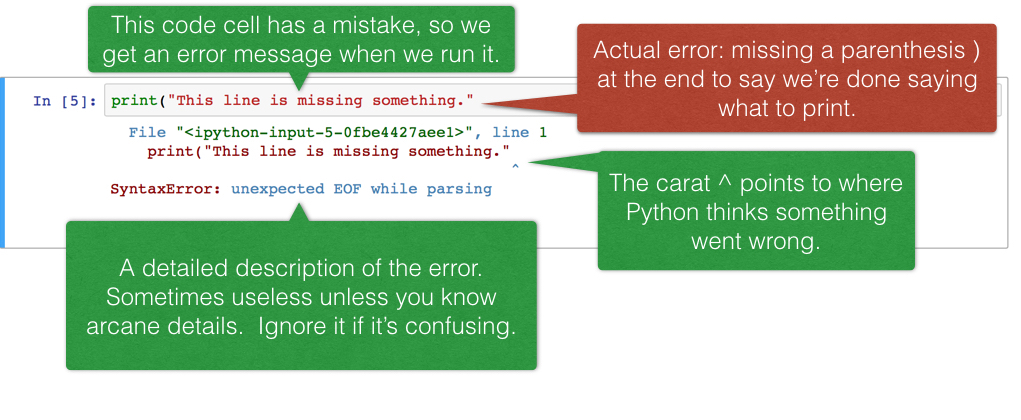
\includegraphics{./images/error.jpg}
\caption{error}
\end{figure}

Fix this error in the cell below:

    \begin{Verbatim}[commandchars=\\\{\}]
{\color{incolor}In [{\color{incolor} }]:} \PY{c+c1}{\PYZsh{}Your Answer Here}
        \PY{o}{.}\PY{o}{.}\PY{o}{.}
\end{Verbatim}


    \begin{center}\rule{0.5\linewidth}{\linethickness}\end{center}

\textbf{Congratulations!} You have completed the introduction to Jupyter
Notebooks tutorial! In the next tutorial, we will use these new skills
to develop further explore data structures like lists, arrays, and
dataframes; and explore statistical concepts like percentiles,
histograms, and standard deviations.

\begin{center}\rule{0.5\linewidth}{\linethickness}\end{center}

\textbf{Sources}

Composing Programs: https://www.composingprograms.com/\\
UC Berkeley Data 8 Textbook :https://inferentialthinking.com\\
UC Berkeley Data Science Education Program - Modules:
https://github.com/orgs/ds-modules/


    % Add a bibliography block to the postdoc
    
    
    
    \end{document}
